% ================================================================= ĐỐI CHUẨN POWER-MF CHẠY LẠI
\subsection{Đối chuẩn với Power-MF chạy lại}
\label{sec:powermf}

\begin{canhbao}[title={RÚT LẠI --- mọi con số Power-MF của bản 3.3 đều sai, kể cả kết luận}]
Bản 3.3 của chính đề cương này, viết sáng 12/09/2026, báo cáo \xau{Power-MF đạt 94,87} trên 18 bản ghi
chung và kết luận rằng \xau{một phần nhỏ hỏng vì ``hai bản ghi bắt cách nhịp''}, rồi loại hai bản ghi đó
để ra con số \xau{98,38 so với 97,33, hiệu số $-1{,}06$}. \textbf{Cả hai đều sai.}

Sai vì cả hai đứng trên một bản Power-MF \textbf{hỏng do lỗi cổng chuyển của chính nhóm}, không phải do
thuật toán. Hàm \texttt{findpeaks} của gói \texttt{signal} trong Octave cài ràng buộc
\texttt{MinPeakDistance} bằng một \textbf{ma trận khoảng cách đôi một} giữa các ứng viên đỉnh, tức
$O(k^2)$ bộ nhớ. Bản ghi Silesia B1 dài 1.197.800 mẫu, sau khi cắt đôi và nội suy $\times 4$ thành
2.395.600 mẫu ở 4000\,Hz, sinh ra hàng chục nghìn ứng viên; ma trận vượt giới hạn chỉ số của Octave và
ném lỗi \texttt{out of memory or dimension too large}. Khối \texttt{try/catch} nội bộ của
\texttt{PowerMF.m} nuốt lỗi đó. MATLAB --- nền tảng tác giả dùng --- giải ràng buộc này bằng thuật toán
tham $O(k \log k)$ nên \textbf{không bao giờ gặp}.

Chữ ký ``Se $\approx$ 50\,\%, PPV $\approx$ 99,7\,\%'' mà nhóm đọc thành ``bắt cách nhịp'' thật ra là
\textbf{mất đúng một nửa bản ghi}: B1\_01 dò được 1.555 đỉnh, \textbf{toàn bộ nằm ở nửa đầu}, 0 đỉnh ở
nửa sau; B1\_02 thì ngược lại, 0 đỉnh nửa đầu và 1.424 đỉnh nửa sau. Nửa nào chạy được thì chạy hoàn
hảo: khoảng cách dò được trung vị 385,5\,ms so với RR thật 386,0\,ms.

Và giả thuyết đầu tiên của nhóm --- \textit{``\texttt{ms\_minpeakdistance} $= 340$\,ms quá sát khoảng RR
thai''} --- \xau{đã bị bác bỏ bằng số đo}. Nhóm đo RR thật từ nhãn tham chiếu
(\texttt{baselines/powermf\_rr\_diag.json}): trên B1\_01, tỉ lệ khoảng RR ngắn hơn 340\,ms là
\textbf{0,00\,\%}. Trên cả 27 bản ghi đã kiểm tra, giá trị lớn nhất là 0,15\,\%. Ràng buộc 340\,ms
\textbf{chưa từng chặn một nhịp thật nào}.
\end{canhbao}

\subsubsection{Bài học phương pháp: nhóm đã phát biểu nguyên nhân trước khi đo}

Đây là chỗ đáng nói nhất của mục này, và nhóm để nó lên trước cả bảng số.

Khi thấy Power-MF hỏng trên 6 bản ghi B1, nhóm đã \textit{đoán} ngay một nguyên nhân nghe rất hợp lý:
tham số 340\,ms quá sát nhịp tim thai 155 nhịp/phút. Giả thuyết đó khớp với trực giác, khớp với con số
nhịp tim, và \textbf{sai}. Nhóm chỉ biết nó sai sau khi bỏ ra một buổi đọc \textit{log} Octave từng bản
ghi và đo phân bố RR thật. Nguyên nhân thật nằm ở một chi tiết cài đặt của thư viện, không nằm ở tham số
nào của thuật toán.

Cái giá của lần đoán sai đó không nhỏ. Nếu nhóm tin vào giả thuyết 340\,ms, nhóm sẽ \textit{chỉnh tham
số} cho Power-MF chạy được, và mọi so sánh về sau sẽ là so với một Power-MF \textbf{đã bị nhóm sửa tham
số} --- một baseline không còn đối chiếu được với bài gốc. Nhóm đã suýt làm đúng như vậy.

Nguyên tắc rút ra, nhóm áp dụng cho toàn bộ phần còn lại của đề tài: \textbf{không phát biểu nguyên nhân
trước khi đo được nguyên nhân}. Một bản ghi hỏng thì đọc \textit{log} của chính nó, không suy diễn từ
tham số. Chi tiết đầy đủ ở \S\ref{sec:doansai}.

\subsubsection{Bản vá P7 và cách nó tái lập ngữ nghĩa MATLAB}

\texttt{baselines/octave/findpeaks\_mpd.m} thay \texttt{findpeaks(x, 'MinPeakDistance', d)} bằng đúng
ngữ nghĩa MATLAB: tìm mọi cực đại địa phương, sắp theo biên độ giảm dần, rồi tham lam nhận đỉnh cao nhất
và loại mọi đỉnh cách nó dưới $d$. Cài bằng \textbf{danh sách liên kết đôi} nên mỗi ứng viên bị gỡ đúng
một lần, tổng chi phí $O(k)$ và không cần ma trận nào. Đo thật: 2.395.600 mẫu chạy trong 14,3\,s.

Kiểm chứng đối chiếu \texttt{baselines/octave/test\_fpmpd.m}, 48 trường hợp: tập đỉnh của
\texttt{findpeaks} Octave \textbf{luôn là tập con} của \texttt{findpeaks\_mpd}, đúng 48/48. Chênh lệch
đến từ bộ lọc bề rộng đỉnh mặc định của Octave (\texttt{MinPeakWidth}, ước lượng bằng khớp parabol) mà
MATLAB \textbf{không có} khi chỉ truyền \texttt{MinPeakDistance}. Nghĩa là P7 kéo bản Octave
\textbf{lại gần} bản MATLAB gốc, chứ không đẩy ra xa. Vì P7 đổi ngữ nghĩa, \textbf{toàn bộ 27 bản ghi đã
được chạy lại} bằng cùng một bản mã.

Tham số \texttt{ms\_minpeakdistance} \textbf{giữ nguyên 340\,ms}, đúng giá trị mặc định của tác giả, ở
mọi lần chạy trong mục này. Nhóm không sửa một tham số nào của Power-MF.

\begin{ghichu}[title={Kiểm chứng ngoài --- bằng chứng mạnh nhất rằng cổng chuyển giờ đã đúng}]
Số \textbf{đã công bố} của chính tác giả cho Silesia B1 là \textbf{99,46} (nhóm trích từ
\texttt{Results/*.mat} của kho gốc, lưu ở \texttt{baselines/powermf\_published.json}).
Sau bản vá P7, nhóm chạy lại trên đúng 10 bản ghi đó và được \tot{99,40 $\pm$ 0,51}.

\textbf{Lệch 0,06 điểm F1.}

Đây là kiểm chứng \textbf{ngoài}: con số đối chiếu do người khác công bố, trên máy khác, bằng MATLAB,
trước khi nhóm bắt tay vào bài toán này. Nhóm không có cách nào ``khớp'' vào nó. Mức lệch 0,06 điểm nằm
trong sai khác biên của \texttt{filtfilt} giữa hai nền tảng. Trước P7, con số tương ứng là \xau{88,19}
và chỉ trên 6 bản ghi chạy được --- lệch \textbf{11,3 điểm}.

Nói cách khác: bản chạy lại \textbf{đã sai 11,3 điểm và giờ sai 0,06 điểm}. Mọi con số Power-MF trong
đề cương từ đây trở đi đứng trên bản sau.
\end{ghichu}

\subsubsection{Ba cột: Power-MF đa kênh, Power-MF đơn kênh, và \hethong{}}

Để trả lời được câu hỏi thật của đề tài, một cột Power-MF là không đủ. Nhóm cài thêm
\textbf{Power-MF-1ch}: chính bộ dò của Jaeger 2024 nhưng chạy ở chế độ \textbf{đơn kênh}.

\begin{ghichu}[title={Power-MF-1ch --- đối chứng công bằng nhất trong cả đề tài}]
Cài bằng Python/scipy thuần (\texttt{baselines/powermf\_1ch.py}), đặc tả lấy từ 21 bước đọc trực tiếp
\texttt{PowerMF.m} (\texttt{survey/scout\_baselines.md} mục 3). Giữ nguyên:
\begin{itemize}[leftmargin=1.5em,itemsep=2pt]
\item nội suy $\times 4$ trước khi dò, đúng như bản gốc;
\item bao hình \textbf{đạo hàm} của tín hiệu dư;
\item mẫu nhịp mẹ bằng \textbf{trung vị} các nhịp đã căn;
\item \textbf{bộ lọc phối hợp} với mẫu fQRS, và \texttt{ms\_minpeakdistance} $= 340$\,ms.
\end{itemize}
Bỏ đúng hai khối, vì cả hai \textbf{bắt buộc phải có nhiều kênh}: \texttt{FecgICAm} và
\texttt{FecgICAf}. Quy tắc chọn kênh theo mật độ phổ công suất của tác giả được thay bằng
\textbf{chính quy tắc PSD mù nhãn của nhóm}, để hai bên chọn kênh giống hệt nhau.

Front-end và bộ khử mẹ dùng \textbf{cùng một hàm} với mô hình của nhóm: \texttt{M.preprocess}
(10--60\,Hz, notch 50\,Hz, hạ về 250\,Hz) và \texttt{M.cancel\_maternal} (mẫu trung vị $+$ bình phương
tối thiểu từng nhịp). Chấm bằng \texttt{M.match\_events}, dung sai $\pm$50\,ms, ghép tham lam 1--1 ---
\textbf{không} dùng \texttt{Bxb\_compare} của kho gốc, để hai bên không thể khác nhau vì bộ chấm.

Vì vậy cột Power-MF-1ch là đối chứng \textbf{sạch nhất} nhóm có: cùng dữ liệu, cùng đạo trình, cùng tiền
xử lý, cùng khử mẹ, cùng bộ chấm. \textbf{Khác biệt duy nhất còn lại là thuật toán lõi} --- bộ lọc phối
hợp cổ điển so với mạng nơ-ron 113.481 tham số.
\end{ghichu}

\begin{table}[H]\centering\small
\caption{F1 trung bình (\%) trên 22 chủ thể, chấm bằng cùng một bộ chấm ($\pm$50\,ms, ghép tham lam
1--1). Nguồn: \texttt{baselines/powermf\_fair\_stats.json} và \texttt{baselines/powermf\_1ch.json}.
Hai cột giữa là \textbf{cùng một thuật toán}, chỉ khác số đạo trình được dùng.}
\label{tab:pmf_bacot}
\begin{tabular}{@{}L{4.4cm} C{0.8cm} C{3.0cm} C{3.0cm} C{3.0cm}@{}}
\toprule
\textbf{Tập} & $n$ & \textbf{Power-MF} \newline \textbf{4 đạo trình} &
\textbf{Power-MF-1ch} \newline \textbf{1 đạo trình} &
\textbf{\hethong{}} \newline \textbf{1 đạo trình} \\
\midrule
ADFECGDB (chuyển dạ) & 5 & $99{,}01 \pm 1{,}05$ & $92{,}37 \pm 2{,}78$ & \tot{$99{,}40 \pm 1{,}01$} \\
Silesia B2 (chuyển dạ) & 7 & $97{,}90 \pm 3{,}77$ & $87{,}28 \pm 18{,}05$ & $96{,}82 \pm 7{,}55$ \\
Silesia B1 (thai kỳ) & 10 & $99{,}40 \pm 0{,}51$ & $83{,}48 \pm 16{,}28$ & $97{,}15 \pm 4{,}95$ \\
\midrule
\textbf{TẤT CẢ 22 chủ thể} & 22 & $\mathbf{98{,}83 \pm 2{,}20}$ & $86{,}71 \pm 14{,}87$ &
$\mathbf{97{,}56 \pm 5{,}30}$ \\
\midrule
CinC 2013 set-a, 60 bản sạch (hệ ghi khác) & 60 & \textit{chưa chạy} & 55,97 & \tot{74,28} \\
\bottomrule
\end{tabular}
\end{table}

Hàng CinC 2013 đáng chú ý riêng. Đó là hệ ghi hoàn toàn khác, không bản ghi nào từng được huấn luyện, và
cả hai phương pháp đơn kênh đều rơi. Nhưng Power-MF-1ch rơi xuống 55,97 còn \hethong{} giữ được 74,28
(hiệu $+18{,}32$, KTC 95\% $[+13{,}35;\ +23{,}64]$, 49 thắng / 5 thua / 6 hoà trên 60 bản sạch; bản 3.4 ghi
62,82 so với 79,40 trên 75 bản, đã rút --- \S\ref{sec:cinc75}).
Nhóm \textbf{chưa chạy} Power-MF 4 kênh trên CinC 2013 --- ô đó để trống, không điền bằng suy đoán.

\begin{table}[H]\centering\small
\caption{F1 từng chủ thể (\%). Cột \hethong{} là mô hình 22 ca, đánh giá bỏ-một-chủ-thể. Ba hàng in đậm
là ba bản ghi \hethong{} thua nặng.}
\label{tab:pmf_tungca}
\begin{tabular}{@{}L{2.0cm} L{2.6cm} C{2.9cm} C{2.9cm} C{2.9cm}@{}}
\toprule
\textbf{Chủ thể} & \textbf{Tập} & \textbf{Power-MF 4 kênh} & \textbf{Power-MF-1ch} &
\textbf{\hethong{}} \\
\midrule
r01 & ADFECGDB & 99,69 & 92,33 & 99,92 \\
r04 & ADFECGDB & 99,53 & 92,41 & 99,68 \\
r07 & ADFECGDB & 99,20 & 90,17 & 100,00 \\
r08 & ADFECGDB & 99,46 & 90,05 & 99,77 \\
r10 & ADFECGDB & 97,15 & 96,91 & 97,61 \\
\midrule
\textbf{B2\_03} & Silesia B2 & \textbf{89,49} & 47,97 & \xau{79,72} \\
B2\_04 & Silesia B2 & 97,95 & 97,88 & 98,90 \\
B2\_05 & Silesia B2 & 99,70 & 90,77 & 100,00 \\
B2\_06 & Silesia B2 & 99,85 & 99,56 & 100,00 \\
B2\_08 & Silesia B2 & 99,77 & 86,13 & 100,00 \\
B2\_09 & Silesia B2 & 98,74 & 98,44 & 99,11 \\
B2\_12 & Silesia B2 & 99,77 & 90,23 & 100,00 \\
\midrule
B1\_01 & Silesia B1 & 99,92 & 95,25 & 99,97 \\
B1\_02 & Silesia B1 & 99,55 & 98,73 & 99,79 \\
B1\_03 & Silesia B1 & 98,97 & 91,30 & 99,92 \\
B1\_04 & Silesia B1 & 99,86 & 99,98 & 100,00 \\
B1\_05 & Silesia B1 & 99,66 & 93,83 & 99,87 \\
\textbf{B1\_06} & Silesia B1 & \textbf{99,97} & 54,36 & \xau{89,45} \\
\textbf{B1\_07} & Silesia B1 & \textbf{99,44} & 63,36 & \xau{86,56} \\
B1\_08 & Silesia B1 & 99,31 & 83,50 & 99,83 \\
B1\_09 & Silesia B1 & 98,39 & 88,27 & 99,07 \\
B1\_10 & Silesia B1 & 98,91 & 66,18 & 97,05 \\
\bottomrule
\end{tabular}
\end{table}

\subsubsection{Thống kê mức chủ thể: ba phép so sánh trên bốn tập con}

Đơn vị phân tích là \textbf{chủ thể}, không phải cặp (bản ghi $\times$ kênh). Khoảng tin cậy 95\% tính
bằng cluster bootstrap 10.000 lần lấy mẫu lại \textbf{chủ thể} có hoàn lại, seed 0. Kèm Wilcoxon ghép
cặp và Cliff $\delta$. Mã: \texttt{baselines/powermf\_fair\_table.py}.

\begin{table}[H]\centering\footnotesize
\caption{Toàn bộ so sánh mức chủ thể. Hiệu số dương nghĩa là phương pháp bên trái cao hơn.
T/H/Th = thắng/hòa/thua theo chủ thể. Nguồn: \texttt{baselines/powermf\_fair\_stats.json}.}
\label{tab:pmf_thongke}
\begin{tabular}{@{}L{2.1cm} L{4.5cm} C{1.4cm} C{2.6cm} C{1.6cm} C{1.1cm} C{1.3cm}@{}}
\toprule
\textbf{Tập} & \textbf{So sánh} & \textbf{Hiệu số} & \textbf{KTC 95\% bootstrap} & $p$ &
\textbf{Cliff} & \textbf{T/H/Th} \\
\midrule
\multirow{3}{*}{Tất cả 22}
 & \hethong{} $-$ Power-MF 4 kênh & $-1{,}27$ & $[-3{,}08;\ +0{,}27]$ & 0,156 & 0,260 & 18/0/4 \\
 & \hethong{} $-$ Power-MF-1ch & \tot{$+10{,}85$} & \tot{$[+6{,}80;\ +15{,}40]$} & $4{,}77\mathrm{e}{-7}$
 & 0,698 & \tot{22/0/0} \\
 & Power-MF-1ch $-$ Power-MF 4 kênh & \xau{$-12{,}12$} & \xau{$[-18{,}27;\ -6{,}90]$} &
 $1{,}43\mathrm{e}{-6}$ & $-0{,}773$ & 1/0/21 \\
\midrule
\multirow{3}{*}{ADFECGDB (5)}
 & \hethong{} $-$ Power-MF 4 kênh & \tot{$+0{,}39$} & \tot{$[+0{,}22;\ +0{,}60]$} & 0,0625 & 0,600 &
 5/0/0 \\
 & \hethong{} $-$ Power-MF-1ch & $+7{,}02$ & $[+3{,}84;\ +9{,}34]$ & 0,0625 & 1,000 & 5/0/0 \\
 & Power-MF-1ch $-$ Power-MF 4 kênh & $-6{,}63$ & $[-8{,}88;\ -3{,}37]$ & 0,0625 & $-1{,}000$ & 0/0/5 \\
\midrule
\multirow{3}{*}{Silesia B2 (7)}
 & \hethong{} $-$ Power-MF 4 kênh & $-1{,}08$ & $[-4{,}04;\ +0{,}54]$ & 0,297 & 0,388 & 6/0/1 \\
 & \hethong{} $-$ Power-MF-1ch & $+9{,}54$ & $[+3{,}09;\ +17{,}87]$ & 0,0156 & 0,673 & 7/0/0 \\
 & Power-MF-1ch $-$ Power-MF 4 kênh & $-10{,}61$ & $[-21{,}84;\ -2{,}67]$ & 0,0156 & $-0{,}673$ &
 0/0/7 \\
\midrule
\multirow{3}{*}{Silesia B1 (10)}
 & \hethong{} $-$ Power-MF 4 kênh & $-2{,}25$ & $[-5{,}55;\ +0{,}32]$ & 1,000 & 0,080 & 7/0/3 \\
 & \hethong{} $-$ Power-MF-1ch & $+13{,}68$ & $[+6{,}91;\ +21{,}27]$ & 0,00195 & 0,620 & 10/0/0 \\
 & Power-MF-1ch $-$ Power-MF 4 kênh & $-15{,}92$ & $[-25{,}93;\ -7{,}05]$ & 0,00391 & $-0{,}780$ &
 1/0/9 \\
\bottomrule
\end{tabular}
\end{table}

Một chi tiết phải đọc đúng. Ở ADFECGDB, KTC 95\% của hiệu số là $[+0{,}22;\ +0{,}60]$ ---
\textbf{không chứa 0}, và thắng 5/5. Nhưng $p$ Wilcoxon là 0,0625, vì với $n = 5$ chủ thể, giá trị $p$
hai phía \textbf{nhỏ nhất có thể đạt} là $2/2^5 = 0{,}0625$. Không phép kiểm định nào trên 5 chủ thể
xuống được dưới 0,05, dù hiệu số lớn đến đâu. Nhóm báo cáo khoảng tin cậy, không tuyên bố ``có ý nghĩa
thống kê'' từ 5 sản phụ.

\begin{figure}[H]\centering
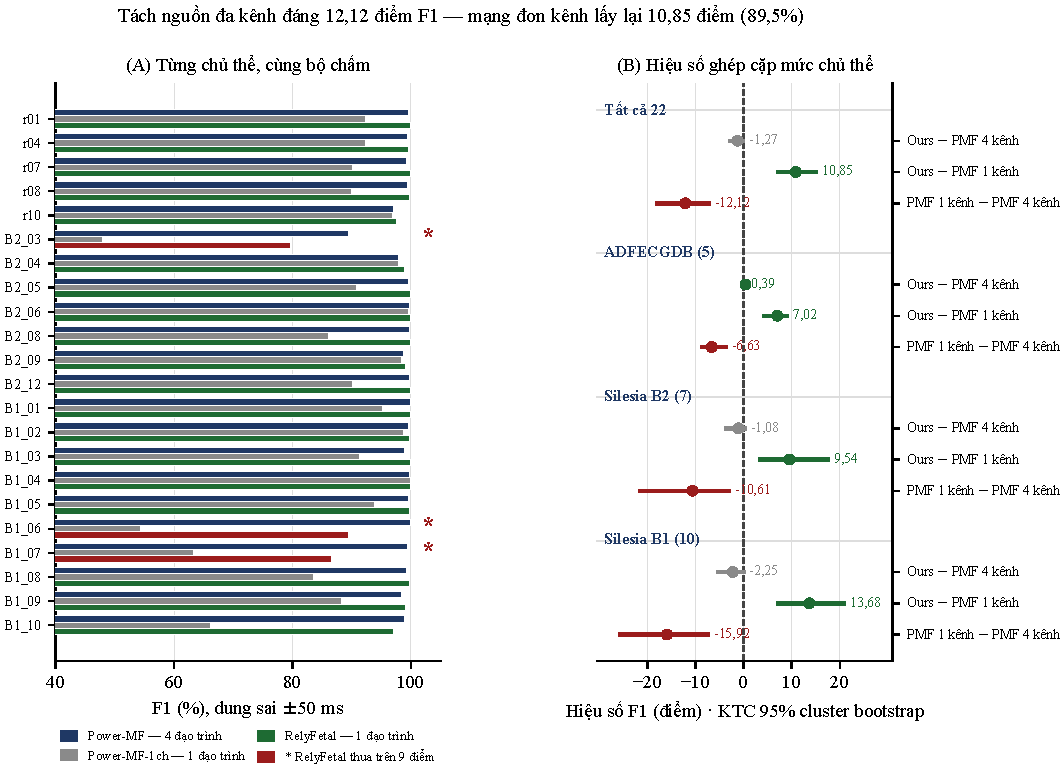
\includegraphics[width=\textwidth]{figs/fig17_powermf.pdf}
\caption{(A) F1 từng chủ thể ở ba cấu hình, cùng bộ chấm $\pm$50\,ms. Ba chủ thể có dấu sao là ba bản
ghi \hethong{} thua nặng --- và Power-MF-1ch cũng sụp ở đúng ba chỗ đó. (B) Hiệu số ghép cặp và KTC 95\%
cluster bootstrap theo tập con, cho cả ba phép so sánh.}
\label{fig:pmf}
\end{figure}

\subsubsection{Ba bản ghi kéo tụt trung bình --- và vì sao phải báo cáo cả trung vị}

\begin{table}[H]\centering\small
\caption{Ba chủ thể \hethong{} thua Power-MF đa kênh quá 9 điểm. Mọi chủ thể còn lại đều thắng, trừ
B1\_10 thua nhẹ.}
\label{tab:pmf_thua}
\begin{tabular}{@{}L{2.0cm} C{2.6cm} C{2.8cm} C{2.2cm} C{3.8cm}@{}}
\toprule
\textbf{Chủ thể} & \textbf{\hethong{}} & \textbf{Power-MF 4 kênh} & \textbf{Hiệu số} &
\textbf{Power-MF-1ch cùng bản ghi} \\
\midrule
B1\_07 & \xau{86,56} & 99,44 & \xau{$-12{,}88$} & 63,36 \\
B1\_06 & \xau{89,45} & 99,97 & \xau{$-10{,}51$} & 54,36 \\
B2\_03 & \xau{79,72} & 89,49 & \xau{$-9{,}77$} & 47,97 \\
\midrule
B1\_10 & 97,05 & 98,91 & $-1{,}86$ & 66,18 \\
\bottomrule
\end{tabular}
\end{table}

Đây là chỗ nhóm phải nói thẳng cả hai mặt, vì cả hai đều thật.

\textbf{Mặt thứ nhất:} nếu nhìn \textbf{trung bình}, \hethong{} \textit{thua} 1,27 điểm F1.
\textbf{Mặt thứ hai:} nếu nhìn \textbf{trung vị}, \hethong{} \textit{hơn} \tot{$+0{,}23$} điểm, và thắng
\tot{18 trên 22} chủ thể.

Hai con số đó không mâu thuẫn. Chúng nói rằng phân bố hiệu số \textbf{lệch mạnh}: đa số chủ thể
\hethong{} hơn một chút, còn ba chủ thể thì thua rất nặng, và ba chủ thể đó một mình kéo trung bình
xuống âm. Trung bình bị ba điểm ngoại lai chi phối; trung vị thì không. Đọc một con số mà bỏ con số kia
đều là đọc sai, nên nhóm báo cáo cả hai ở mọi chỗ.

Nhóm \textbf{không} loại ba bản ghi này. Bài học của bản 3.3 là: loại bản ghi khi chưa hiểu nguyên nhân
thì sẽ ra kết luận sai --- lần đó nhóm loại hai bản ghi và ra con số 98,38 hoàn toàn hư cấu. Lần này ba
bản ghi được giữ nguyên trong mọi phép tính.

Một điều đáng chú ý: trên đúng ba bản ghi đó, \textbf{Power-MF-1ch cũng sụp} --- 63,36 / 54,36 / 47,97,
tức còn tệ hơn \hethong{} nhiều. Nghĩa là đây là ba bản ghi mà \textbf{tín hiệu một đạo trình thật sự
không đủ}, chứ không phải ba bản ghi mà mạng nơ-ron kém. Cả hai phương pháp đơn kênh đều hỏng ở đúng
những chỗ đó, và chỉ tách nguồn đa kênh cứu được. Nhóm xem đây là giới hạn của \textit{cấu hình đơn
kênh}, không phải của \textit{mô hình}. Đó cũng chính là lý do đề tài cần một cổng từ chối trả lời
(\S\ref{sec:fsqi}): khi một đạo trình không đủ, hệ thống phải nói ``không đọc được'' thay vì đưa ra một
nhịp tim sai.

\subsubsection{Luận đề đúng của đề tài: lấy lại 89,5\,\% lợi ích của đa kênh bằng một kênh}
\label{sec:luande}

Câu hỏi mà mục này thật sự trả lời không phải ``ai hơn ai''. Nó là:

\begin{quote}
\textit{Một mạng \textbf{đơn kênh} 113.481 tham số lấy lại được bao nhiêu phần của lợi ích mà
\textbf{tách nguồn đa kênh} mang lại?}
\end{quote}

Câu hỏi này đo được, vì nhóm có cả ba cột.

\begin{enumerate}[leftmargin=1.8em,itemsep=5pt]
\item \textbf{Tách nguồn đa kênh đáng bao nhiêu?} Lấy \textit{chính} Power-MF và bỏ hai khối ICA đa kênh
đi: $98{,}83 \rightarrow 86{,}71$. Mất \xau{12,12 điểm F1}, KTC 95\% $[-18{,}27;\ -6{,}90]$,
$p = 1{,}43\mathrm{e}{-6}$, thua 21/22 chủ thể. Đây là \textbf{giá của đa kênh}, đo trên cùng một thuật
toán nên không lẫn với bất kỳ khác biệt nào khác.
\item \textbf{Mô hình đơn kênh lấy lại bao nhiêu?} Trên cùng một đạo trình, \hethong{} hơn Power-MF-1ch
\tot{10,85 điểm}, KTC 95\% $[+6{,}80;\ +15{,}40]$, $p = 4{,}77\mathrm{e}{-7}$, thắng \tot{22/22} chủ
thể.
\item \textbf{Tỉ lệ:} $10{,}85 / 12{,}12 = \mathbf{89{,}5\,\%}$. Mạng đơn kênh lấy lại gần chín phần
mười lợi ích của tách nguồn đa kênh, \textbf{bằng một đạo trình duy nhất}.
\end{enumerate}

Hệ quả: trên 22 chủ thể độc lập, \hethong{} \textbf{không phân biệt được} với Power-MF đa kênh
($-1{,}27$ điểm; KTC 95\% $[-3{,}08;\ +0{,}27]$; $p = 0{,}156$), và \textbf{hơn hẳn} Power-MF khi
Power-MF bị giới hạn về cùng một đạo trình ($+10{,}85$ điểm; 22/22).

\begin{ghichu}[title={Phát biểu đúng --- đây là câu nhóm sẽ dùng trong bài báo, nguyên văn}]
\textit{``Trên 22 chủ thể độc lập, chấm bằng cùng một giao thức ($\pm$50\,ms, ghép tham lam 1--1), bỏ
hai khối ICA đa kênh khỏi Power-MF làm chính nó mất 12,12 điểm F1 (KTC 95\% cluster bootstrap
$[-18{,}27;\ -6{,}90]$). Một mô hình đơn kênh 113.481 tham số lấy lại 10,85 điểm trong số đó
(KTC 95\% $[+6{,}80;\ +15{,}40]$; Wilcoxon $p = 4{,}77\mathrm{e}{-7}$; thắng 22/22 chủ thể), tức
\textbf{89,5\,\% lợi ích của tách nguồn đa kênh, bằng một đạo trình duy nhất}. So với Power-MF đa kênh
đầy đủ, hiệu số là $-1{,}27$ điểm (KTC 95\% $[-3{,}08;\ +0{,}27]$; $p = 0{,}156$; trung vị hiệu số
$+0{,}23$; thắng 18/22) --- \textbf{không phân biệt được}.''}
\end{ghichu}

\begin{canhbao}[title={Ba điều KHÔNG được nói kèm phát biểu trên}]
\begin{enumerate}[leftmargin=1.6em,itemsep=4pt]
\item \textbf{Không nói ``vượt trội'', ``SOTA'', hay ``đầu tiên''.} Trên B2 và B1, hiệu số so với
Power-MF đa kênh là \textbf{âm}; Power-MF nhỉnh hơn, chỉ là khoảng tin cậy vẫn chứa 0. Trên trung bình
toàn tập \hethong{} \textit{thua} 1,27 điểm. ``Không phân biệt được'' là cụm từ đúng; ``hơn'' thì không.
\item \textbf{Không nói Power-MF yếu trên thai kỳ.} Power-MF đạt 99,40 trên Silesia B1 --- cao hơn
\hethong{} 2,25 điểm, và gần như trùng số công bố của chính tác giả. Mọi ấn tượng ngược lại ở bản 3.3
là do lỗi cổng chuyển của nhóm, và đã được rút ở hộp đầu mục này.
\item \textbf{Không nói 89,5\,\% là một hằng số.} Nó là tỉ số giữa hai hiệu số ước lượng, mỗi hiệu số có
khoảng tin cậy riêng khá rộng. Nhóm \textbf{chưa} tính KTC cho chính tỉ số này. Cách phát biểu an toàn
là ``phần lớn, khoảng chín phần mười''. Nhóm không viết ``89,5\,\% $\pm$ gì đó'' vì chưa đo được sai số
đó.
\end{enumerate}
\end{canhbao}

\subsubsection{Ý nghĩa với định vị của cả đề tài}

Trước mục này, C1 (đối chuẩn công bằng) dựa vào một con số trích từ y văn. Giờ nó dựa vào ba cột tự đo
trên cùng một máy, cùng dữ liệu, cùng bộ chấm --- và một trong ba cột tái lập được số công bố của tác
giả đến 0,06 điểm.

Quan trọng hơn: nhóm không còn phải tranh luận ``học sâu có thắng xử lý tín hiệu cổ điển không''. Câu
hỏi đó \textbf{sai ngay từ cách đặt}, vì hai bên không dùng cùng số đạo trình. Câu hỏi đúng là câu hỏi ở
\S\ref{sec:luande}, và nó có câu trả lời bằng số: 89,5\,\%.

Điều \hethong{} mua được so với Power-MF đa kênh không phải là F1 cao hơn. Đó là: \textbf{một đạo trình
thay vì bốn} --- một miếng dán đeo được tại nhà, thay vì một bộ điện cực bụng cần kỹ thuật viên đặt đúng
vị trí; 113.481 tham số và 4,35\,ms mỗi cửa sổ 4 giây; và một cổng từ chối trả lời, thứ mà Power-MF
không có, cũng không cần, vì Power-MF không được thiết kế để chạy không giám sát.
